\documentclass[a4paper]{ctexart}
\pagestyle{plain}
\usepackage{amsmath}
\usepackage{amssymb}
\usepackage{graphicx}
\usepackage{tikz}
\usetikzlibrary{patterns}
\title{\textbf{Assigment 2 for Combinational Mathmatics}}
\date{2020.9.24}
\author{Guo Yuhang \\ 202021080728
}
\begin{document}
\maketitle
\section*{Exercise 2}
 %1,2,3,4,7,8,9,10,11,13,14,16,20
 
 1.求从$1-10000$的整数中,不能够被$3,4,5$中任意一个整除的整数的个数。\\
 \textbf{Solution:} 定义全集为$S$表示从1到10000的所有整数的集合,定义$p_1$表示满足整数能够被3整除这一性质;定义$p_2$表示满足整数能够被4整除这一性质;定义$p_3$表示满足整数能够被5整除这一性质。同时分别定义$A_1,A_2,A_3$表示满足性质$p_1,p_2,p_3$的所有整数的集合。那么根据容斥原理,在$1-10000$的所有整数中不能被$3,4,5$中任意一个整除的整数总数可以表示为:
 \[
\begin{split}
|\bar{A}_1\cap \bar{A}_2\cap \bar{A}_3|&=|S|-(|A_1|+|A_2|+|A_3|)\\ 
&+(|A_1\cap A_2|+|A_1\cap A_3|+|A_2\cap A_3|)-(|A_1\cap A_2|\cap A_3)\\
&=10000-(3333+2500+2000)+(833+666+500)-166\\
&=4000
\end{split} 
 \]
因此最终在$1-10000$的整数中共有$4000$个整数不能够被$3,4,5$中任意一个整除。

2. 求$1-1000$中既非完全平方又非完全立方的整数的个数。\\
\textbf{Solution:} 定义全集$S$表示为从1到1000的所有整数的集合。定义$p_1$表示在$1-1000$中满足是完全平方的整数;定义$p_2$表示在$1-1000$中满足完全立方的整数。同时定义$A_1,A_2$为分别满足$p_1,p_2$性质的整数的集合。根据容斥原理我们可以知道,在$1-1000$中既非完全平方数又非完全立方数的整数个数可以表示为:
\[
\begin{split}
|\bar{A}_1\cap\bar{A}_2| &= |S|-(|A_1|+|A_2|)+(|A_1|\cap |A_2|)\\
&= 1000 - (31+10)+3\\
&=962
\end{split}
\]
因此最终在$1-1000$中的整数既非完全平方又非完全立方的整数的个数为962个。

3. 某校学生共有120名参加了数学竞赛,竞赛试题共有甲乙丙三题。竞赛的结果是12名同学3题全对;20名同学只做对了甲乙两题;16名同学做对了甲丙两题;28名同学做对了乙丙两题;48名同学做对了甲题;56名同学做对了乙题;16名同学三题都做错了,试求出做对了丙题的学生人数。\\
\textbf{Solution:} 假设$p_1$表示只做对甲题这一性质;$p_2$表示只做对乙题这一性质;$p_3$表示只做对丙题这一性质。分别使用集合$A_1,A_2,A_3$表示这三种性质对应的学生集合。\\
根据题中已给数据和容斥原理我们可以写出:
\[
\begin{aligned}
|\bar{A}_1\cap \bar{A}_2\cap \bar{A}_3|&=|S|-(|A_1|+|A_2|+|A_3|)\\ 
&+(|A_1\cap A_2|+|A_1\cap A_3|+|A_2\cap A_3|)-(|A_1\cap A_2|\cap A_3)\\
16&=120 -(48+56+|A_3|)+(20+12+16+28)-12\\
\end{aligned}
\]
解出方程我们可以得到$|A_3|=64$. 因此做对了丙题的学生人数为64人。

4. 在有10个字母$a,a,b,b,c,c,d,d,e,e$的全排列中,求相同字母不相邻的排列个数。\\
\textbf{Solution:} 定义全集$S$为这10个字母全排列组成的集合,定义$p_1$表示字母$a$在排列中一定相邻的情况;定义$p_2$表示字母$b$在排列中一定相邻的情况;定义$p_3$表示字母$c$在排列中一定相邻的情况;定义$p_4$表示字母$d$在排列中一定相邻的情况;定义$p_5$表示字母$e$在排列中一定相邻的情况。那么根据容斥原理我们可以知道所有相同字母不相邻的排列数可以表示为:$|\bar{A}_1\cap\bar{A}_2\cap\bar{A}_3\cap \bar{A}_4\cap \bar{A}_5|$. \\
对于$|A_i|$,我们可以将相同字母绑定后进行排列,可以看作9个字母的重集的全排列$9!/2!2!2!2!1!$. 对于$|A_i\cap A_j|$可以看成两组字母绑定后的全排列
\[
\begin{split}
&|\bar{A}_1\cap\bar{A}_2\cap\bar{A}_3\cap \bar{A}_4\cap \bar{A}_5|\\ =& |S|-\sum_{i=1}^5 |A_i| 
+ \sum_{i\neq j}|A_i\cap A_j| -\cdots +(-1)^5 |A_1\cap A_2\cap A_3\cap A_4\cap A_5|\\ 
=&\frac{10!}{2!2!2!2!2!}-\binom{5}{1}\frac{9!}{2!2!2!2!1!}+\binom{5}{2}\frac{8!}{2!2!2!1!1!}\\
-&\binom{5}{3}\frac{7!}{2!2!1!1!1!}+\binom{5}{4}\frac{6!}{2!1!1!1!1!}-\binom{5}{5}\frac{5!}{1!1!1!1!1!}\\
=&113400-5\times 22680+10\times 5040-10\times 1260+5\times 360-120\\
=&39480\\
\end{split}
\]
因此我们可以知道在这10个字母中相同字母不相邻的排列个数为39480个。

7. 在由26个字母$a,b,c\cdots,z$组成的全排列中,求不包含字符串$john$, $paul$, $smite$的全排列个数。\\
\textbf{Solution:} 假设全集$S$表示的是由这26个字母组成的所有全排列情况,同时设$p_1$表示包含字符串$john$这一性质的字符串;设$p_2$表示的是包含字符串$paul$这一性质的字符串;设$p_3$表示的是包含字符串$smite$这一性质的字符串。同时分别定义$A_1,A_2,A_3$表示满足$p_1,p_2,p_3$三个性质的字符串的集合。根据容斥原理我们可以将不包含$john,paul,smite$这三个字符串的字符串的集合可以写为:$|\bar{A}_1\cap \bar{A}_2\cap \bar{A}_3|$. \\
计算过程如下:
\[
\begin{split}
&|\bar{A}_1\cap \bar{A}_2\cap \bar{A}_3|\\
=&|S|-(|A_1|+|A_2|+|A_3|)+(|A_1\cap A_2|+|A_1\cap A_3|+|A_2\cap A_3|)-(|A_1\cap A_2\cap A_3|)\\
=& 26! -23!-23!-22!+20!+19!+19!-16!\\
=& 26! - 2\times 23! -22! +20!+2\times 19! -16!
\end{split}
\]

8. 在所有的$n$位数中,包含数字$3,8,9$但不包含$0,4$的数有多少个。\\
\textbf{Solution:} 首先不包含0,4我们可以直接将0,4排除在外,也就是说$1,2,3,5,6,7,8,9$这8个数进行排列。首先假设全集$S$表示由这8个数组成的排列情况,设$p_1$表示组成的数字中包含3的情况;$p_2$表示组成的数字中包含8的情况;$p_3$表示组成的数字中包含9的情况。对应的集合分别为$A_1,A_2,A_3$.根据容斥原理我们可以知道:
\[
\begin{split}
&|\bar{A}_1\cap \bar{A}_2\cap \bar{A}_3|\\
=&|S|-(|A_1|+|A_2|+|A_3|)+(|A_1\cap A_2|+|A_1\cap A_3|+|A_2\cap A_3|)-(|A_1\cap A_2\cap A_3|)\\
=& 8^n-3\times 7^n + 3\times 6^n -5^n\\
\end{split}
\]
因此满足条件的数一共有$8^n-3\times 7^n + 3\times 6^n -5^n$个。

9. 一个体育团体共25人,其中14人会踢足球,12人会打乒乓球,6人既会打乒乓球又会踢足球,5人既会打篮球又会踢足球,还有2对这三种球都会打,而6个会打篮球的人都会打另外一种球(这三种球的一种)。求不会打球的人数。\\
\textbf{Solution:} 定义全集$S$表示的是整个体育团体中的所有人,定义$p_1$表示会踢足球的人,$p_2$表示会打乒乓球的人,$p_3$表示会打篮球的人。$A_1,A_2,A_3$分别对应具有这三种性质的人的集合。那么三种球都不会的人的集合可以表示为:$\bar{A}_1\cap \bar{A}_2\cap \bar{A}_3$.根据鸽笼原理我们可以写出下面的表达式:
\[
\begin{split}
&|\bar{A}_1\cap \bar{A}_2\cap \bar{A}_3|\\
=&|S|-(|A_1|+|A_2|+|A_3|)+(|A_1\cap A_2|+|A_1\cap A_3|+|A_2\cap A_3|)-(|A_1\cap A_2\cap A_3|)\\
=& 25-(14+12+6) +(6+5+6) -2\\
=& 25-32 +17 - 2\\
=& 8
\end{split}
\]
因此在这个体育团体中存在8个人这三种球都不会打。

10. 求重集$B=\{3\cdot a,4\cdot b,5\cdot c\}$.\\
\textbf{Solution:} 重新定义一个重集$B'=\{\infty \cdot a,\infty \cdot b, \infty \cdot c\}$. 定义$p_1$表示排列中至少包含4个a,定义$p_2$表示排列中至少包含5个b,定义$p_3$表示排列中至少包含6个c. 同时分别定义满足这三种性质的排列的集合为$A_1,A_2,A_3$. 那么原重集的10-组合数可以表示为:$\bar{A}_1\cap\bar{A}_2\cap\bar{A}_3$. 根据容斥原理我们可以进行求解:
\[
\begin{split}
&|\bar{A}_1\cap \bar{A}_2\cap \bar{A}_3|\\
=&|S|-(|A_1|+|A_2|+|A_3|)+(|A_1\cap A_2|+|A_1\cap A_3|+|A_2\cap A_3|)-(|A_1\cap A_2\cap A_3|)\\
=& F(3,10)-(F(3,6)+F(3,5)+F(3,4))+(F(3,1)+F(3,0)+0)-0\\
=& 66-(28+21+15)+(3+1+0)-0\\
=&6
\end{split}
\]
因此重集$B=\{3\cdot a,4\cdot b,5\cdot c\}$的10-组合数为6.

11. 求重集$B=\{\infty \cdot a,3\cdot b,5\cdot c,7\cdot d\}$的10-组合数。\\
\textbf{Solution:} 重新定义一个重集$B'=\{\infty \cdot a,\infty \cdot b,\infty \cdot c,\infty \cdot d\}$.设由重集$B'$构成的10-组合数为$S$.定义$p_1$表示排列至少包含11个a,同时$A_1$集合表示满足这一条件的所有排列情况组合的集合;定义$p_2$表示排列至少包含4个b,同时$A_2$集合表示满足这一条件的所有排列情况组合的集合;定义$p_3$表示排列至少包含6个c,同时$A_3$集合表示满足这一条件的所有排列情况组合的集合;定义$p_4$表示排列至少包含8个d,同时$A_4$集合表示满足这一条件的所有排列情况组合的集合. 根据容斥原理我们可以写出:
\[
\begin{split}
&|\bar{A}_1\cap \bar{A}_2\cap \bar{A}_3\cap\bar{A}_4|\\
=&|S|-\sum_{i=1}^{4}|A_i|+\sum_{i\neq j} |A_i\cap A_j| -\sum_{i\neq j\neq k}|A_i\cap A_j\cap A_k|+|A_1\cap A_2\cap A_3\cap A_4|\\
=& F(4,10) -(0+F(4,6)+F(4,4)+F(4,2))+F(4,0)\\
=& 286-84-35-10+1\\
=& 158
\end{split}
\]
因此重集$B=\{\infty \cdot a,3\cdot b,5\cdot c,7\cdot d\}$的10-组合数为158.

13. 求由数字$1,2,\cdots,8$所组成的全排列中偶数均不在其自然位置上的全排列的个数。\\
\textbf{Solution:} 根据题意,我们需要考虑的问题是$2,4,6,8$不在原位置的情况,其他的4个数随便排列。因此我们可以定义全集$S$为这8个数组成的全排列,同时假设$p_1$表示数字$2$排列在原位置的排列;假设$p_2$表示数字$4$排列在原位置的排列;假设$p_3$表示数字$6$排列在原位置的排列;假设$p_4$表示数字$8$排列在原位置的排列。分别假设对应的集合为$A_1$表示数字2在原位置的排列集合,$A_2$表示数字4在原位置的排列集合,$A_3$表示数字6在原位置的排列集合,$A_4$表示数字8在原位置的排列集合。根据容斥原理可以写出:
\[
\begin{split}
&|\bar{A}_1\cap\bar{A}_2\cap\bar{A}_3\cap\bar{A}_4|\\
=& |S|-\sum_{i=1}^4|A_i|+\sum_{i\neq j}|A_i\cap A_j|-\sum_{i\neq j\neq k}|A_i\cap A_j\cap A_k|+|A_1\cap A_2\cap A_3\cap A_4|\\
=& 8! - \binom{4}{1}7! + \binom{4}{2} 6! -\binom{4}{3} 5!+\binom{4}{4}4! \\
=&24024
\end{split}
\]
因此由数字$1,2\cdots,8$所组成的全排列中偶数均不在其自然位置上的全排列的个数为24024.

14. 求由数字$1,2,\cdots,8$所组成的全排列中,恰好有4个数字在其自然位置上的全排列个数。\\
\textbf{Solution:} 根据错排的公式我们可以直接写出结果:
\[
\begin{split}
D_4 \binom{8}{4} &= 4!\binom{8}{4}\left[ 1-\frac{1}{1!}+\frac{1}{2!}-\frac{1}{3!}+\frac{1}{4!} \right]\\
&=\frac{8!}{4!}\left[ 1-1+\frac{1}{2}-\frac{1}{6}+\frac{1}{24} \right]\\
&= 630
\end{split}
\]
因此由数字$1,2,\cdots,8$所组成的全排列中,恰好有4个数字在其自然位置上的全排列的个数为630个。

16. 证明:$D_n$是偶数当且仅当$n$是奇数。\\
\textbf{Solution:} 当$n=1$时,$D_n=0$; 当$n$为大于1的奇数的情况下,我们设$n=2k-1$, 其中$k=2,3,\cdots$. 则$D_n=D_{2k-1}$. 根据推论$D_n=(n-1)(D_{n-1}+D_{n-2})$. 将$n=2k-1$代入其中,我们可以得到:$D_{2k-1}=2(k-1)(D_{2k-2}+D_{2k-3})$. 其中$k$取从2开始的一系列正整数。从而我们不难发现无论$(k-1)(D_{2k-2}+D_(2k-3))$取任意的整数值得到的$D_{2k-1}$表示的一定是一个偶数。

20. 有张、王、刘、李4位教师和数学,物理,化学,英语4门课程。已知张和李都不能教数学和英语,王不能教化学,刘不能教物理和化学。若要为每人安排一门他能教的课程,且一门课程只能被一个人教,试问有多少种不同的安排方案?\\
\textbf{Solution:} 在考虑这种存在一般限制的排列问题时,我们可以使用棋盘多项式的方式来进行求解。使用棋盘多项式求解的顺序为:(1)画出带有一般限制的棋盘;(2)求解$R(C_n)$;(3)利用$n$元有禁位的排列数公式进行求解:$n!-r_1(n-1)!+r_2(n-2)!-\cdots+(-1)^nr_n$求解结果。下面我们先画出棋盘:
\begin{figure}[!htbp]
\centering
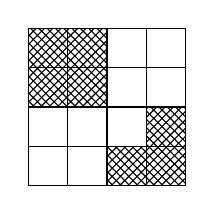
\begin{tikzpicture}
\draw[step=0.5] (0,0) grid (2,2);
\pattern[pattern=crosshatch] (0,2) rectangle (0.5,1.5);
\pattern[pattern=crosshatch] (0,1.5) rectangle (0.5,1);
\pattern[pattern=crosshatch] (0.5,2) rectangle (1,1.5);
\pattern[pattern=crosshatch] (0.5,1.5) rectangle (1,1);
\pattern[pattern=crosshatch] (1.5,1) rectangle (2,0.5);
\pattern[pattern=crosshatch] (1.5,0.5) rectangle (2,0);
\pattern[pattern=crosshatch] (1,0.5) rectangle (1.5,0);
\end{tikzpicture}
\caption{有禁位棋盘结构}
\end{figure}

根据棋盘我们将棋盘分解为两个独立的棋盘$C_1,C_2$.因此我们得到的棋盘多项式可以写为:
\[
\begin{split}
R(C)&=R(C_1)R(C_2)\\
&=(1+4x+2x^2)(1+3x+x^2)\\
&=1+7x+15x^2+10x^3+2x^4\\
\end{split}
\]
带入$n$元有禁位的排列数公式进行求解:$n!-r_1(n-1)!+r_2(n-2)!-\cdots+(-1)^nr_n$可以计算结果:
\[
N=4! - 7\times 3! +15\times 2!-10\times 1!+2=4
\]
因此共有4种不用的排课方案。
\end{document} 